%%%%%%%%%%%%%%%%%%%%%%%%%%%%%%%%%%%%%%%%%%%%%%%%%%%%%%%%%%%%%%%%%%%%%%%%%%%%%%%%
\chapter{Introdução à Programação}
\label{cap:un1}


%%%%%%%%%%%%%%%%%%%%%%%%%%%%%%%%%%%%%%%%
\section{Lab 1: Jogo Clique no Alonzo}
\label{cap:un1-lab1}

Neste Lab (laboratório de programação) você programará um aplicativo (app) que
poderá compartilhar com outras pessoas e jogar em seu telefone.


%%%%%%%%%%%%%%%%%%%%
\subsection{Atividade 1: começando com o \snap}
\label{cap:un1-lab1-01}

Nesta seção você aprenderá como criar sua própria conta no \snap, como fazer o
\ingles{login} (entrar) e o \ingles{logout} (sair).

%%%%%%%%%%
\subsubsection{Criando uma conta}
\label{cap:un1-lab1-01-a}

\begin{enumerate}
\item Se você ainda não abriu o \snap, abra agora:
      \url{https://snap.berkeley.edu/}.

\item Na janela do \snap, clique no menu \ingles{Cloud} (nuvem),
      \inlinefigure{imagens/cloud\_button.png}, selecione
      \ingles{Signup}\ldots\ (inscrever-se), e siga as instruções.
\end{enumerate}

\begin{figure}[H]
\centering
%\caption{}
%\label{fig:}
%\fbox{
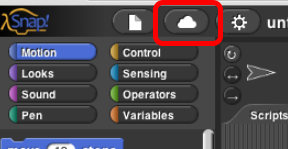
\includegraphics[scale=0.5]{imagens/button-cloud-with-context.png}
\hspace{4cm}
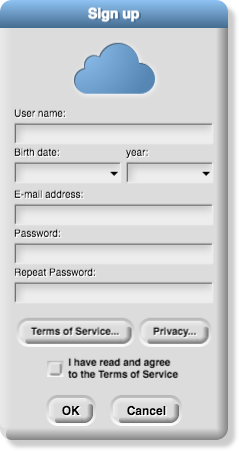
\includegraphics[scale=0.35]{imagens/dialog-cloud-signup.png}
%}\\
%\footnotesize{Fonte: xxx}
\end{figure}

Você terá que clicar em um link em seu e-mail para verificar sua conta, mas não
precisa fazer isso agora nesse momento. A qualquer momento você pode alterar sua
senha clicando no menu \ingles{Cloud},
\inlinefigure{imagens/cloud\_button.png}.

%%%%%%%%%%
\subsubsection{Entrando e saindo de sua conta no \snap}
\label{cap:un1-lab1-01-b}

Você deve estar logado sempre que estiver no \snap. Veja como verificar se você
está logado:

\begin{enumerate}[resume]
\item Clique no menu \ingles{Cloud}.
      \begin{itemize}
      \item \textbf{Se} estiver mostrando ``\ingles{Logout}'' e o seu nome de
            usuário, então você já está logado.
      \item \textbf{Se} estiver aparecendo o nome de outra pessoa, então saia
            e entre novamente com seu usuário.
      \item \textbf{Caso contrário}, escolha ``\ingles{Login}'' e entre com o
            seu nome de usuário e sua senha.
      \end{itemize}
\item Lembre-se de sair do \snap\ quando você terminar suas atividades!
\end{enumerate}

Observação: você pode clicar no botão da engrenagem,
\inlinefigure{imagens/engine.png}, e alterar a linguagem do \snap\ para
português. Não aconselhamos você a fazer isso para que você vá se acostumando
com os termos utilizados em programação, que são todos em inglês mesmo.
